% Created 2016-04-04 Mon 15:09
% Intended LaTeX compiler: pdflatex
\documentclass[11pt]{article}
\usepackage[utf8]{inputenc}
\usepackage[T1]{fontenc}
\usepackage{graphicx}
\usepackage{grffile}
\usepackage{longtable}
\usepackage{wrapfig}
\usepackage{rotating}
\usepackage[normalem]{ulem}
\usepackage{amsmath}
\usepackage{textcomp}
\usepackage{amssymb}
\usepackage{capt-of}
\usepackage{hyperref}
\usepackage{minted}
\usepackage[margin=0.5in]{geometry}
\author{Bachir El khadir}
\date{\textit{<2016-03-11 Fri>}}
\title{Problem set 5, ORF525}
\hypersetup{
 pdfauthor={Bachir El khadir},
 pdftitle={Problem set 5, ORF525},
 pdfkeywords={},
 pdfsubject={},
 pdfcreator={Emacs 25.1.50.1 (Org mode )}, 
 pdflang={English}}
\begin{document}

\maketitle
\begin{HTML}

\label{orgspecialblock1}

\end{HTML}


\section{Q1}
\label{sec:orgheadline3}

\subsection{Helper function to remove 0s from final table}
\label{sec:orgheadline1}

\begin{minted}[frame=lines,linenos=true]{r}
n <- 19
  replace.zeros <- function(X){
      X2 <- as.matrix(X)
      for(j in 1:n) {
          for(k in 1:n) {
              if(X[j, k] != 0) next
              kmax = k-1
              jmax = j-1
              kmin = k+1
              jmin = j+1
              while(kmax > 0 && X[j, kmax] ==0) kmax = kmax-1
              while(jmax > 0 && X[jmax, k] ==0) jmax = jmax-1
              while(kmin <= n && X[j, kmin] == 0) kmin = kmin+1
              while(jmin <= n && X[jmin, k] == 0) jmin = jmin+1

              average <- 0
              if(kmax > 0) average <- average + X[j, kmax]
              if(jmax > 0) average <- average + X[jmax, k]
              if(kmin <= n) average <- average + X[j, kmin]
              if(jmin <= n) average <- average + X[jmin, k]
              X2[j, k] = sign(average)
          }
      }
      X2
  }
\end{minted}







\subsection{Load the data from file}
\label{sec:orgheadline2}
\begin{minted}[frame=lines,linenos=true]{r}
library(ptw)
setwd('~/Documents/Princeton/ORF525/hw5/')

load.game <- function(file, replace) {
    game <-read.table(file, header=F, sep=",")
    if(replace)
        game <- replace.zeros(game)
    game
}

move80.files <- list.files('2014Games/Games_Move80', full.names = T)
final.files <- list.files('2014Games/Games_Final', full.names = T)

cat("Load Move 80 Games\n")
move80.games <- lapply(move80.files, function(f) load.game(f, F))

cat("Load Final Games\n")
final.games <- lapply(final.files, function(f) load.game(f, T))

length(move80.games)
\end{minted}




\textbf{1.2}

We have that:

\begin{align*}
\mathcal L_n(\theta) &= -\frac1K \sum_i \log P_{\theta}(s_i | c_i)
\\&= \frac1K \sum_i \log Z(\theta, c_i) - f(s_i, c_i, \theta)
\end{align*}

So:

\begin{align*}
\frac{\partial \mathcal L_n}{\partial \theta}
= \frac1K \sum_i \frac{\partial \log Z(\theta, c_i)}{\partial \theta}
- \frac1K \sum_i  \frac{\partial f(\theta, c_i, s_i)}{\partial \theta}
\end{align*}

But:

\begin{align*}
E_{s \sim P_{\theta}(s | c_i)}[ \frac{\partial f(s, c_i, \theta)}{\partial \theta}]
\\&=  \int \frac{\partial}{\partial \theta} f(s, c_i, \theta) P_{\theta}(s | c_i) ds
\\&=  \frac1{Z(c_i, \theta)} \int \frac{\partial f(s, c_i, \theta)}{\partial \theta} e^{f(s, c_i, \theta)} ds
\\&=  \frac1{Z(c_i, \theta)} \int \frac{\partial}{\partial \theta} e^{f(s, c_i, \theta)} ds
\\&=  \frac1{Z(c_i, \theta)} \frac{\partial}{\partial \theta} \int  e^{f(s, c_i, \theta)} ds
\\&=  \frac1{Z(c_i, \theta)} \frac{\partial}{\partial \theta} \int Z(c_i, \theta) P_{\theta}(s | c_i)  ds
\\&=  \frac1{Z(c_i, \theta)} \frac{\partial Z(c_i, \theta)}{\partial \theta}
\\&= \frac{\partial \log Z(c_i, \theta)}{\partial \theta} 
\end{align*}

Which means that:

\begin{align*}
\frac{\partial \mathcal L_n}{\partial \theta}
= \frac1K \sum_i E_{s \sim P_{\theta}(s | c_i)}[ \frac{\partial f(s, c_i, \theta)}{\partial \theta}]
- \frac1K \sum_i  \frac{\partial f(\theta, s_i, c_i)}{\partial \theta}
\end{align*}



\begin{minted}[frame=lines,linenos=true]{r}
library(IsingSampler)

n <- 19
neighbours <- t(array(c( 1,0, 0, 1, -1, 0, 0, -1), c(2, 4)))
# theta: w_chains, w_winterchain, w_chainempty, w_empty, h_stones

weight <- function(cj, ck, theta) {
    if(cj == ck & cj != 0) return(theta[1])
    if(cj == -ck & cj != 0) return(theta[2])
    if(cj*ck == 0 & cj+ck != 0) return(theta[3])
    return(theta[4])
}

gradient.weight <- function(cj, ck, theta) {
    r <- array(0, dim=length(theta))
    i <- 0
    if(cj == ck & cj != 0) i <- 1
    else if(cj == -ck & cj != 0) i <- 2
    else if(cj*ck == 0 & cj+ck != 0) i <- 3
    else i <- 4
    r[i] <- 1
    r
}

gradient.threshold <- function(){
    c(0, 0, 0, 0, 1)
}

sample.ising <- function(num, c, theta){
    c <- as.matrix(c)
    graph <- array(0, c(n, n, n, n))
    thresholds <- array(0, c(n, n))
    for(a in 1:n) 
        for(b in 1:n)
            for(i in 1:4) {
                x <- a + neighbours[i, 1]
                y <- b + neighbours[i, 2]
                if(x < 1 | y < 1 | x > n | y > n) next
                cj = c[[a, b]]
                ck = c[[x, y]]
                graph[a, b, x, y] = weight(cj, ck, theta)
                thresholds[a, b] = thresholds[a, b] + cj * theta[5]
                thresholds[x, y] = thresholds[x, y] + ck * theta[5]
            }
    graph <- array(graph, dim=c(n*n, n*n))
    thresholds <- array(thresholds, dim=c(n*n))
    IsingSampler(num, -graph, -thresholds, nIter=20, responses=c(-1, 1))
}

gradient.f <- function(c, s, theta) {
    c <- as.matrix(c)
    s <- as.matrix(s)
    grad <- array(0, dim=length(theta))
    for(a in 1:n) 
        for(b in 1:n)
            for(i in 1:4) {
                x <- a + neighbours[i, 1]
                y <- b + neighbours[i, 2]
                if(x < 1 | y < 1 | x > n | y > n) next
                cj = c[[a, b]]
                ck = c[[x, y]]
                sj = s[[a, b]]
                sk = s[[x, y]]
                grad <- grad + sj*sk*gradient.weight(cj, ck, theta) + (sj*cj+ sk*ck) * gradient.threshold()
            }
    grad
}


gradient.MLE <- function(final.games, move80.games, theta, M=10) {
    grad <- 0 * theta
    K <- length(move80.games)
    for(i in 1:K) {
        c <- move80.games[[i]]
        sample <- sample.ising(M, c, theta)
        grad <- grad + rowMeans(sapply(1:M, function(j) gradient.f(c, array(sample[j, ], c(n, n)), theta))) 

        s <- final.games[[i]]
        grad <- grad - gradient.f(c,s,theta)
    }

    (grad/K)
}

gradient.descent <- function(final.games, move80.games, theta0, M=5, rate=0.001) {
    theta <- theta0
    niter <- 20
    for(i in 1:niter) {
        delta <- gradient.MLE(final.games, move80.games, theta, M)
        theta <- theta - rate * delta
        cat(paste(i, crossprod(delta), "\n"))
        cat("theta:\n")
        cat(theta)
        cat("\n")
    }
    theta
}
\end{minted}


\begin{minted}[frame=lines,linenos=true]{r}
gradient.descent(final.games, move80.games, theta0, M=5, rate=0.001)
\end{minted}

After performing the MLE, we get the following value for \(\theta\)

\begin{center}
\begin{tabular}{rrrrr}
\hline
-1.70 & 6.39 & 0.89 & 23.43 & 15.63\\
\hline
\end{tabular}
\end{center}


\textbf{1.3}
Function to plot the board:
\begin{minted}[frame=lines,linenos=true]{r}
plt.board <- function(s, s.expected) {
c0 <- array(as.matrix(s), c(n*n))
expectation  <- 10 * array(as.matrix(s.expected), c(n*n))
plot(1:19,type="n",xlim=c(1,19),axes=F,xlab='',ylab='',bty="o",lab=c(19,19,1))
rect(par("usr")[1],par("usr")[3],par("usr")[2],par("usr")[4],col = "gray")
rect(1,1,2:19,2:19)
rect(1:18,1:18,19,19)
for (i in 1:19) {
    position=rep(23,19)
    color=rep("black",19)
    for (j in 1:19)  {
        if (abs(c0[19*(i-1)+j])==1) {
            position[j]=20-i
            if (c0[19*(i-1)+j]==-1) color[j]="white"
        }
    }
    points(position,cex=3,pch=21,bg=color)
}

for (i in 1:19) {
    position=rep(20-i,19)
    color=rep("black",19)
    for (j in 1:19) 
        if (expectation[19*(i-1)+j]<=0) color[j]="white"
    points(position,cex=1.5*abs(expectation[(19*(i-1)+1):(19*i)]),pch=22,bg=color,col=color)

}

}
\end{minted}


Predict the result of the game:
\begin{minted}[frame=lines,linenos=true]{r}
theta.hat <- c(-1.70 , 6.39 , 0.89 , 23.43 , 15.63)
predict.board <- function(c, theta, M=100) {
    sample <- sample.ising(M, c, theta)
    array(rowMeans(sample), c(n, n))
}

move80.test.files <- c("AlphaGo-vs-Lee/AlphaGo-vs-Lee-game2_80.txt","AlphaGo-vs-Lee/AlphaGo-vs-Lee-game4_80.txt")
final.test.files <- c("AlphaGo-vs-Lee/AlphaGo-vs-Lee-game2_final.txt","AlphaGo-vs-Lee/AlphaGo-vs-Lee-game4_final.txt")

move80.test.games <- lapply(move80.test.files, function(f)load.game(f, replace=F))
final.test.games <- lapply(final.test.files, function(f)load.game(f, replace=T))
predict <- lapply(move80.test.games, function(s) predict.board(c, theta.hat))

players <- c("white", "black")
predict.game <- function(i){
    w <- sum(final.test.games[[i]]) - 3.75
    w.predict <- sum(predict[[i]]) - 3.75
    plt.board(final.test.games[[i]], predict[[i]])
    title(paste("real winner:", players[(w>0)+1], "predicted winner:", players[(w.predict > 0) + 1]))
}
\end{minted}


Plot the results:

\begin{minted}[frame=lines,linenos=true]{r}
predict.game(1)
\end{minted}

\begin{center}
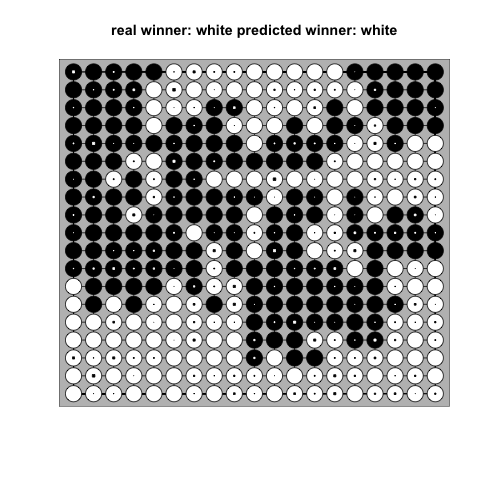
\includegraphics[width=.9\linewidth]{img/game1.png}
\captionof{figure}{game 1}
\end{center}

\begin{minted}[frame=lines,linenos=true]{r}
predict.game(2)
\end{minted}

\begin{center}
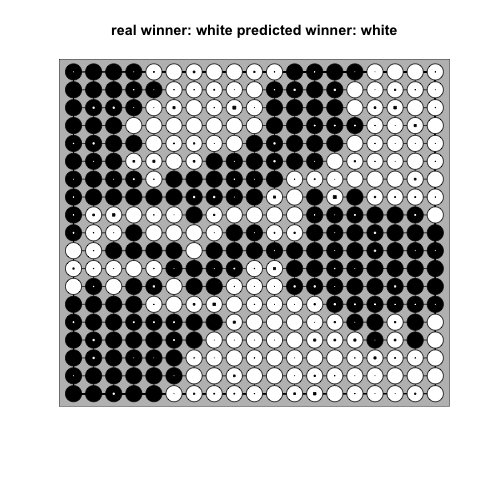
\includegraphics[width=.9\linewidth]{img/game2.png}
\captionof{figure}{game 2}
\end{center}





\section{Q2}
\label{sec:orgheadline4}

\textbf{2.1}
\begin{align*}
P(Y = 1 | X = x)
&= \frac{P(X = x | Y = 1)P(Y = 1)}{P(X = x)}
\\&= \frac{P(X = x | Y = 1)P(Y = 1)}{P(X = x)}
\\&= \frac{P(X = x | Y = 1)P(Y = 1)}{P(X = x|Y=1)P(Y=1)+P(X = x|Y=-1)P(Y=-1)}
\\&= \frac{P(X = x | Y = 1)}{P(X = x|Y=1)+P(X = x|Y=-1)\frac{P(Y=-1)}{P(Y=1)}}
\\&= \frac{ e^{-\gamma_1 x}}{e^{-\gamma_1 x}+ \frac{\gamma_0}{\gamma_1}e^{-\gamma_0 x}\frac{P(Y=-1)}{P(Y=1)}}
\\&= \frac{e^{\beta_1 x + \beta_0}}{1 + e^{\beta_1 x + \beta_0}}
& (\beta_1 = \gamma_0 - \gamma_1 , e^{-\beta_0} = \frac{\gamma_0}{\gamma_1}\frac{P(Y=-1)}{P(Y=1)})
\end{align*}



\textbf{2.2}

\textbf{part a}
\begin{minted}[frame=lines,linenos=true]{r}
library(ggplot2)

logistic <- function(x, beta=1, beta0=1)  (1 / (1 + exp(-beta * x - beta0)))
x <- seq(-20, 20, 0.1)
eta <- logistic(x)
eta2 <- logistic(x, beta0=2)

p1 <- ggplot(NULL, aes(x=x, y=eta)) +
    geom_line() +
    ggtitle("With bias")

p2 <- ggplot(NULL, aes(x=x, y=eta2)) +
    geom_line() +
    ggtitle("Without bias")

multiplot(p1, p2)
\end{minted}

\begin{center}
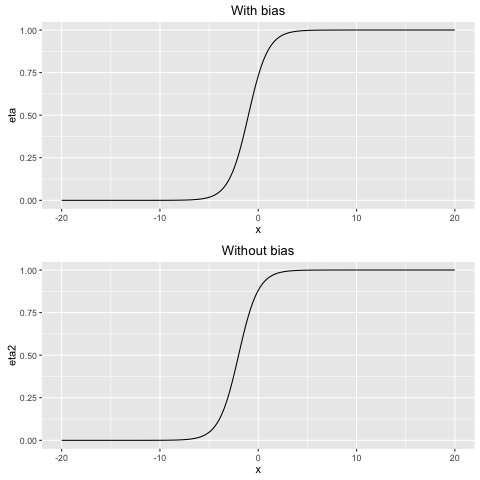
\includegraphics[width=.9\linewidth]{logistic.png}
\captionof{figure}{Comparaison}
\end{center}


Without a bias \(\beta_0\) force \(\eta(x)\) to be symmetric around \(\frac12\) when \(x\) is symmetric around \(0\), e.g \(\eta(-x) = 1 - \eta(x)\)

\textbf{part b}

\begin{align*}
\log P_{\beta}(X, Y)
&= \sum \log P(X_i, Y_i)
\\&= \sum \log P_{\beta}(Y_i | X_i) + \log P(X_i)
\\&= \sum \log \mathcal B(\eta(X_i))(Y_i) + cte
\\&= \sum \log \eta(X_i) 1_{Y_i=1} + (1-\eta(X_i))1_{Y_i = 0} + \log P(X)
\\&= \sum_{Y_i=1} \log \eta(X_i) + \sum_{Y_i=0} \log (1 - \eta(X_i)) + \log P(X)
\\&= \sum_{Y_i=1} \log \eta(X_i) + \sum_{Y_i=0} \log \eta(-X_i) + \log P(X)
\end{align*}

\textbf{part c}

In this case, $$P_{\beta}(X, Y) = \sum_i \log \eta(-|X_i|) + cte$$

Where we use the fact that \(\forall x > 0\;  \log \eta(x) =  \log \frac1{1+e^{-\beta x}}\) is strictly increasing as a function of \(\beta\), and when \(x = 0\), \(\eta(x)\) doesn't depend on \(\beta\), so the maximum of the sum is attained when \(\hat \beta = \infty\)


\textbf{2.3}

$$\frac{\beta^{\alpha}}{\Gamma(\alpha)} x^{\alpha-1} e^{-\beta x} = \frac{\alpha^{\alpha} x^{\alpha-1}}{\Gamma(\alpha)} e^{\alpha (-\frac{\beta}{\alpha} x +  \log \frac{\beta}{\alpha})}$$

This is
\begin{itemize}
\item \(\theta = -\frac\beta\alpha\)
\item \(A(\theta) = -\log \theta\)
\item \(\lambda = \alpha\)
\item \(h(\lambda, x) = \frac{\lambda^{\lambda} x^{\lambda-1}}{\Gamma(\lambda)}\)
\end{itemize}

the canonical link funciton is then \((A')^{-1}(x) = -(\frac 1x)^{-1} = -\frac 1x\)

\section{Q3}
\label{sec:orgheadline5}

\textbf{a)}

Without loss of generality we can assume:
\begin{itemize}
\item The expectation to be 0 by subtracting the mean of the gaussian vector.
\item \(i = 1, j = 2\)
\end{itemize}

In this case, we can write the density as:
\begin{align*}
f(X_1, \ldots, X_n)
&\propto e^{-\Theta_{1,2}X_1X_2  + g_1(X_{-1}) + g_2(X_{-2})}
\\&\propto e^{-\Theta_{1,2}X_1X_2} e^{g_1(X_{-1})}e^{g_2(X_{-2})} 
\end{align*}
So that:
\(f(X_1, X_2 | X_{-1, -2}) \propto e^{-\Theta_{1,2}X_1X_2} e^{g_1(X_2)} e^{g_2(X_1)}\)

Wich proves that \(X_1 \perp X_2\) conditional on \(X_{-1, -2}\) if and only if \(e^{-\Theta_{1,2}X_1X_2}\) can be decomposed as a product of a function of \(X_1\) and a function of \(X_2\), which is the case if and only if \(\Theta_{1,2} = 0\)


\textbf{b)}
Again let's assume that the mean is 0.

Let \(Z = X_j - \alpha_j^T X_{-j}\)
Then \(\Theta_{jj}Z = \Theta_{jj}X_j - \sum_{k \ne j} \Theta_{j,k} X_k\)


\begin{align*}
\Theta_{jj} cov(Z, X_l)
&= \Theta_{jj} \Sigma_{jl} - \sum_{k \ne j} \Theta_{jk} \Sigma_{k, l}
\\&= \Theta_{jj} \Sigma_{jl} -  (\Theta_j^T \Sigma_l - \Theta_{jj}\Sigma{jl})
\\&= \Theta_j^T \Sigma_l
\\&= (I_d)_{jl} = 0
\end{align*}


When \(l \ne j\), then \(cov(Z, X_l) = 0\).

Since \(X\) is gaussian, this proves that \(Z\) is gaussian and is independent from \(X_{-j}\).
Let's now calculate its variance and mean.

\begin{itemize}
\item \(\mathcal E[Z] = 0\) because it is a linear combination of 0 mean variables \(X_i\).
\item \(cov(Z, Z) = \frac1{\Theta_{jj}} [\underbrace{\Theta_{jj} cov(Z, X_j)}_1 - \sum_{k \le j} \Theta_{jk} \underbrace{cov(Z, X_k)}_0] = \frac1{\Theta_{jj}}\)
\end{itemize}



so \(\epsilon_j := Z \sim \mathcal N(0, \frac1{\Theta_{jj}})\)

\textbf{3.2}

\textbf{a}

Without loss of generality, let's assume that \(j = 1, k = 2\)
Bayes rule:
\begin{align*}
P(x_1, x_2 | X_{-1, -2})
&\propto e^{2 \theta_{12}x_1x_2}  e^{f(x_1)} e^{g(x_2)}
\end{align*}

\(x_1 \perp x_2\) conditional on \(X_{-1, -2}\) if and only if \(P(x_1, x_2 | X_{-1, -2})\) can be decomposed into a product of a function of \(x_1\) times a function of \(x_2\), which the case if and only if \(\theta_{12} = 0\).

\textbf{b}
Without loss of generality, we can assume that \(\theta\) is symmetric by replacing it by \(\tilde \theta \sim \frac{\theta + \theta'}2\).

Bayes rule:
\begin{align*}
p(x_1 | X_{-1})
&\propto e^{\tilde \theta_{11} x_1^2 + 2 x_1\sum_{j \ge 2} \tilde \theta_{12} x_j} 
\\&\propto e^{2 x_1\sum_{j \ge 2} \tilde \theta_{12} x_j} &(x_1^2 = 1)
\\&= \frac{1}{U(\tilde \theta, x_{-1})} e^{2 x_1\sum_{j \ge 2} \tilde \theta_{1j} x_j} 
\end{align*}
To find the constant of proportionality \(U(\tilde \theta, x_{-1})\), we use the fact that a density sums to 1:

$$U(\tilde \theta, x_{-1})=  e^{2 \sum_{j \ge 2} \tilde \theta_{1j} x_j} +e^{-2 \sum_{j \ge 2} \tilde \theta_{1j} x_j}$$


so that:

\begin{align*}
p(x_1 | X_{-1})
&= \frac{1}{U(\tilde \theta, x_{-1})} e^{2 x_1\sum_{j \ge 2} \tilde \theta_{1j} x_j}
\\&= \frac{e^{2 x_1\sum_{j \ge 2} \tilde \theta_{1j} x_j}}{e^{2 \sum_{j \ge 2} \tilde \theta_{1j} x_j} +  e^{-2 \sum_{j \ge 2} \tilde \theta_{1j} x_j}}
\\&= \frac{e^{2 x_1\sum_{j \ge 2} \tilde \theta_{1j} x_j}}{e^{2 x_1\sum_{j \ge 2} \tilde \theta_{1j} x_j} +  e^{-2 x_1\sum_{j \ge 2} \tilde \theta_{1j} x_j}} &\text{(because $x_i = \pm 1$)}
\\&= \frac{e^{4 x_1\sum_{j \ge 2} \tilde \theta_{1j} x_j}}{e^{4 x_1\sum_{j \ge 2} \tilde \theta_{1j} x_j} +  1}
\\&= \frac{e^{2 x_1\sum_{j \ge 2}  \theta_{1j} x_j}}{e^{2 x_1\sum_{j \ge 2}  \theta_{1j} x_j} +  1}
\end{align*}
\end{document}